\documentclass[12pt]{beamer}
\usetheme{AnnArbor}
\setbeamercolor{normal text}{bg=black!10}
\begin{document}
\title{Design of Integrated Microrobotic Fish}
\subtitle{Presentation 2 - Physical Model (Preliminary)}
\author{Yihua Liu}
\institute{UM-SJTU Joint Institute}
\date{March 2, 2021}
\begin{frame}
    \titlepage
\end{frame}
\section{Basic Frame}
\begin{frame}{Basic Frame}
    \begin{columns}[onlytextwidth]
        \begin{column}{0.4\textwidth}
            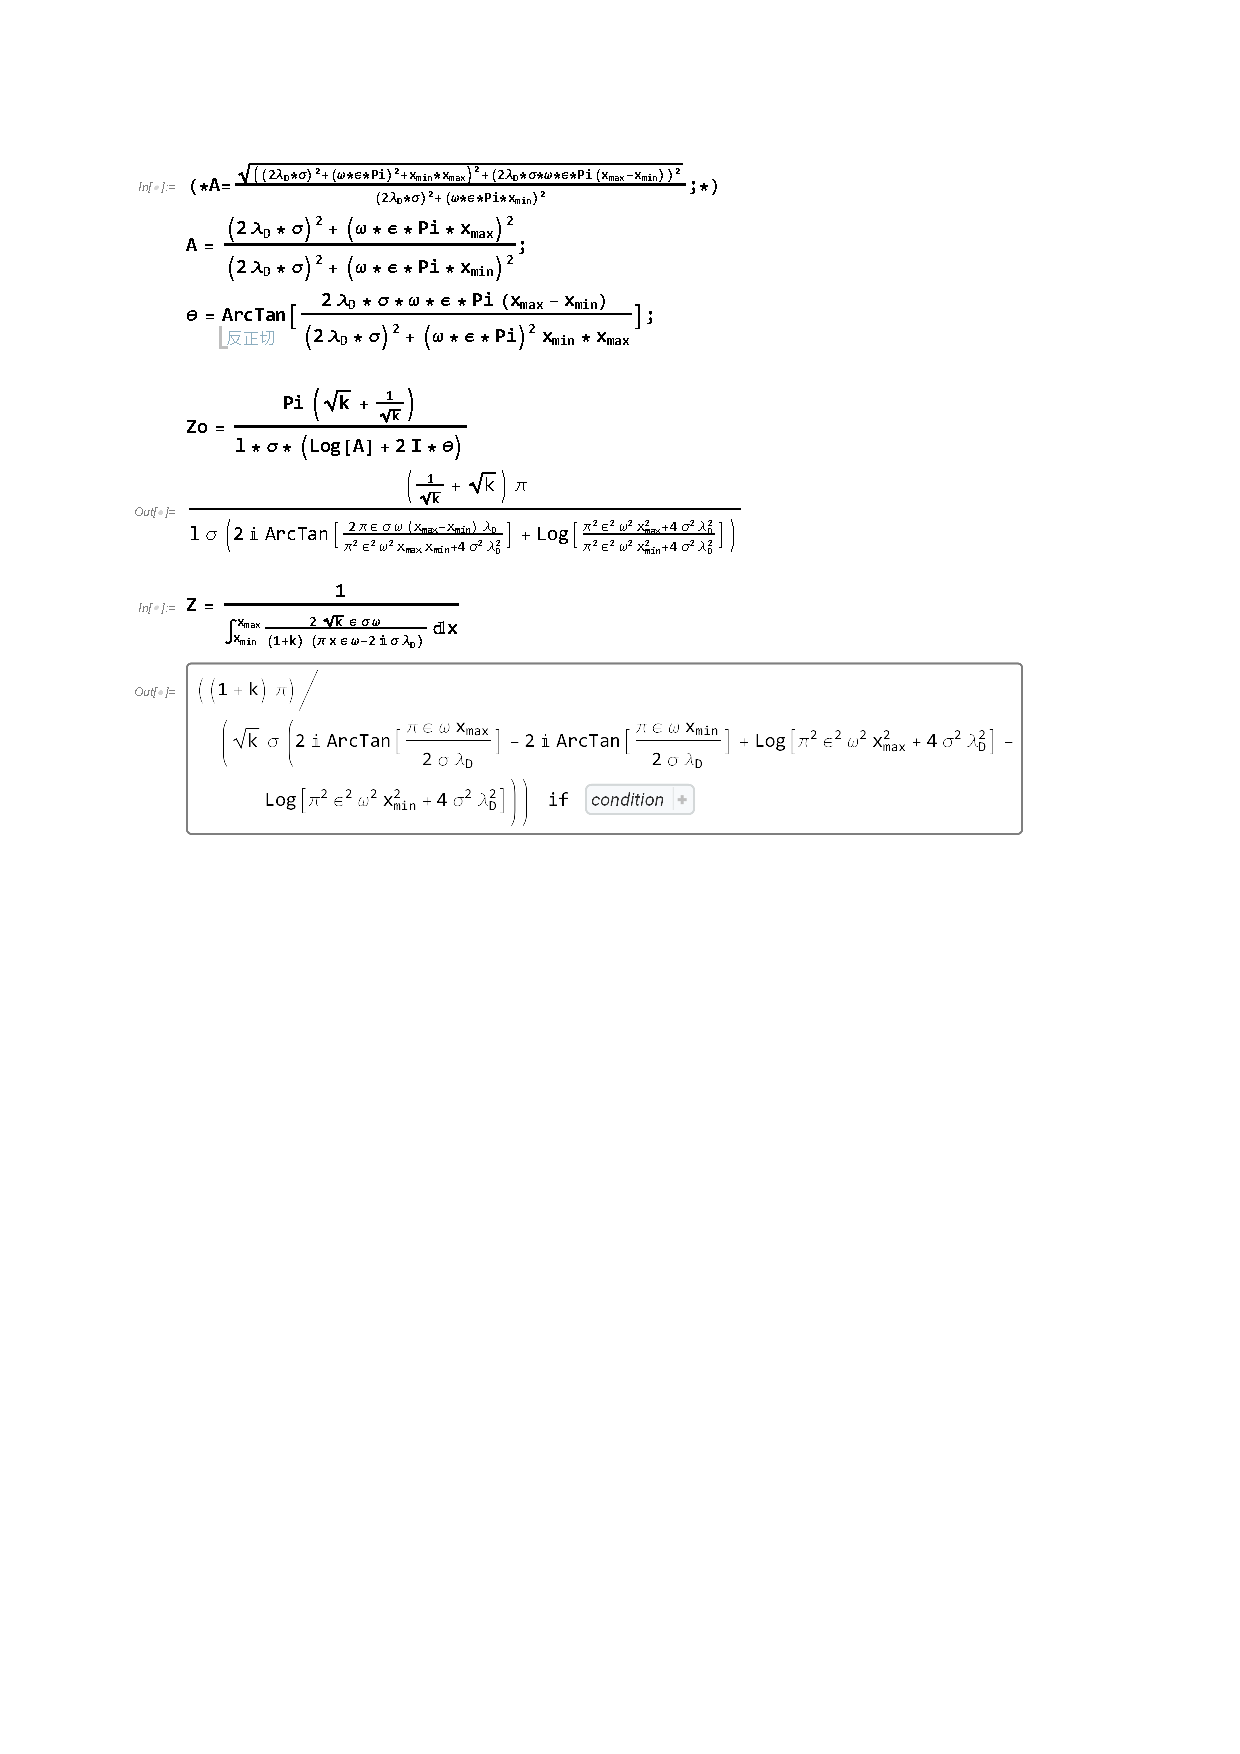
\includegraphics[width=\columnwidth]{1.jpg}
        \end{column}
        \begin{column}{0.6\textwidth}
            \begin{itemize}
                \item The double layers at the electrode surfaces -\textgreater Capacitance\\
                      The capacitance of the double layer at each end of the tube per unit length of the electrode $C_{DL}$ and at the large electrode $C_{DS}$
                \item The bulk water -\textgreater Resistance\\
                      The resistance of the tube per unit length of electrode $R(x)$
            \end{itemize}
        \end{column}
    \end{columns}
\end{frame}
\section{Resistance}
\begin{frame}{Resistance}
    \begin{columns}[onlytextwidth]
        \begin{column}{0.4\textwidth}
            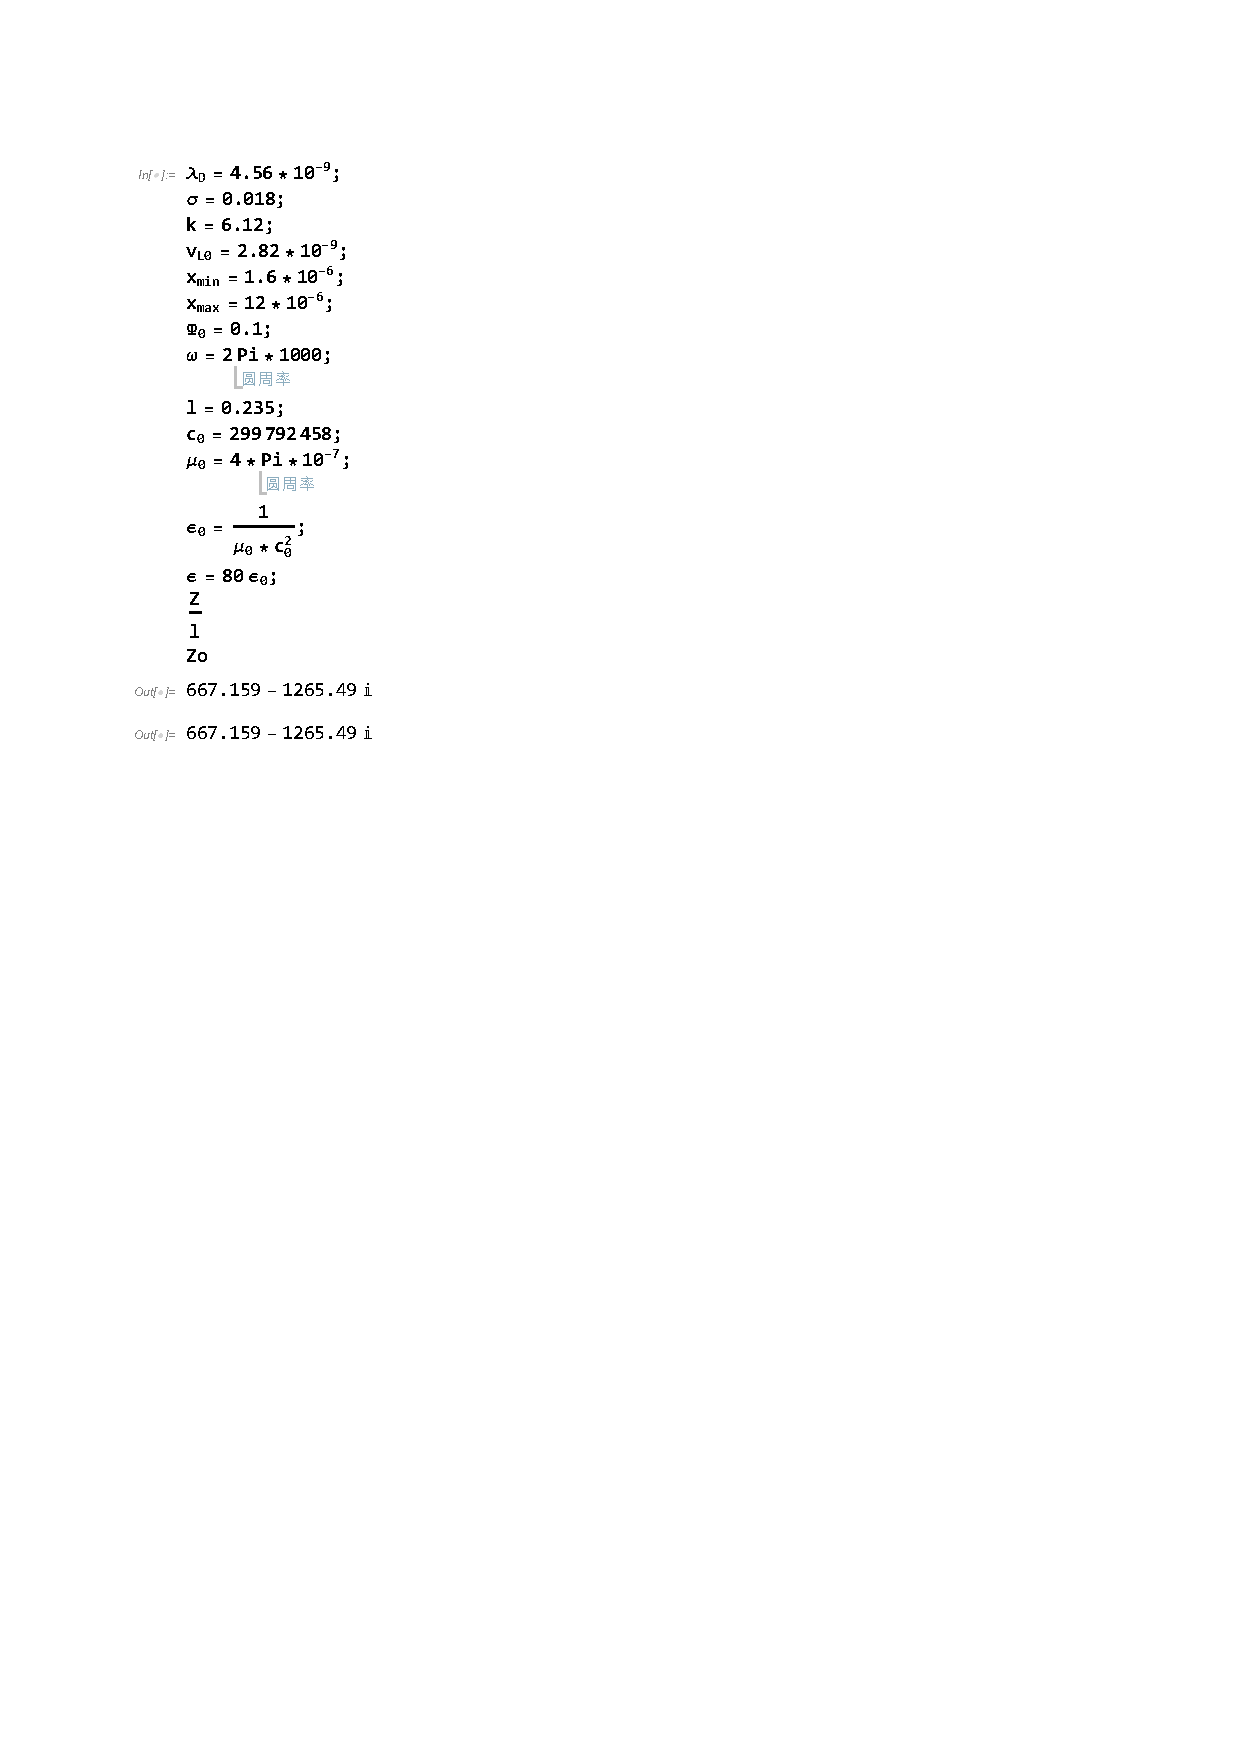
\includegraphics[width=\columnwidth]{2.png}
        \end{column}
        \begin{column}{0.55\textwidth}
            Different form common three-dimensional resistance given by $R=\frac{\rho L}{S}$, here the resistance is two-dimensional given by $R=\frac{\rho L}{d}=\frac{L}{\sigma d}$.\\
            We can take infinitesimals of $x$ ($\delta x$) to calculate $R(x)$. Here we can assume the electric field lines are semicircles, so $L=\pi r$ where the radius $r=\frac{\sqrt{k}+\frac{1}{\sqrt{k}}}{2}$.\\
            Therefore, we have $R(x)=\frac{\pi x\left(\sqrt{k}+\frac{1}{\sqrt{k}}\right)}{2\sigma\delta x}.$
        \end{column}
    \end{columns}
\end{frame}
\section{Capacitance}
\begin{frame}{Capacitance}
    Different form common three-dimensional capacitance given by $C=\frac{\varepsilon S}{d}$, here the resistance is two-dimensional given by $R=\frac{\varepsilon L}{d}$.\\
    Then, we can derive that $C_{DL}=\frac{\varepsilon\delta x\sqrt{k}}{\lambda_D}$ and $C_{DL}=\frac{\varepsilon\delta x}{\sqrt{k}\lambda_D}$.
\end{frame}
\section{Electric Field}
\begin{frame}{Electric Field}
    Now, there are three parts of impedance: $C_{DL}$, $C_{DS}$, and $R(x)$ in total, and the total difference of electric potential is $\Psi=\Psi_0\exp{i\omega t}$.
    Based on two equations:\\
    \[\Psi=I\cdot R_{total}=I(R+\frac{1}{i\omega C_{DL}}+\frac{1}{i\omega C_{DS}})\]
    \[\Psi_{DL}(x)=I\cdot\frac{1}{i\omega C_{DL}}\]
    We have\\
    \[\Psi_{DL}(x)=\Psi-IR-\frac{I}{i\omega C_{DS}}=\frac{\Psi}{1+k}\frac{1}{1+\frac{i\omega\varepsilon\pi x}{2\lambda_D\sigma}}\]
\end{frame}
\begin{frame}{Electric Field}
    Then, by taking the derivative of $\Psi_{DL}(x)$, we have\\
    \[E_{HL}=\frac{1}{\sqrt{k}}\frac{\mathrm{d}\Psi_{DL}}{\mathrm{d}x}=-\frac{\Psi}{\sqrt{k}(1+k)}\frac{\frac{i\omega\varepsilon\pi}{2\lambda_D\sigma}}{(1+\frac{i\omega\varepsilon\pi x}{2\lambda_D\sigma})^2}\]
\end{frame}
\section{Velocity}
\begin{frame}{Velocity}
    Based on the principle of the fluid dynamics, we have the velocity of the ions and the fluid $v_{DL}$ is\\
    \[v_{DL}=\frac{\lambda_D\rho_{DL}E_{HL}}{\eta}\]
    where\\
    \[\rho_{DL}=\frac{\Psi_{DL}C_{DL}}{\delta x\sqrt{k}}=\frac{\Psi_{DL}\varepsilon}{\lambda_D}\]
\end{frame}
\begin{frame}{Velocity}
    \begin{columns}[onlytextwidth]
        \begin{column}{0.55\textwidth}
            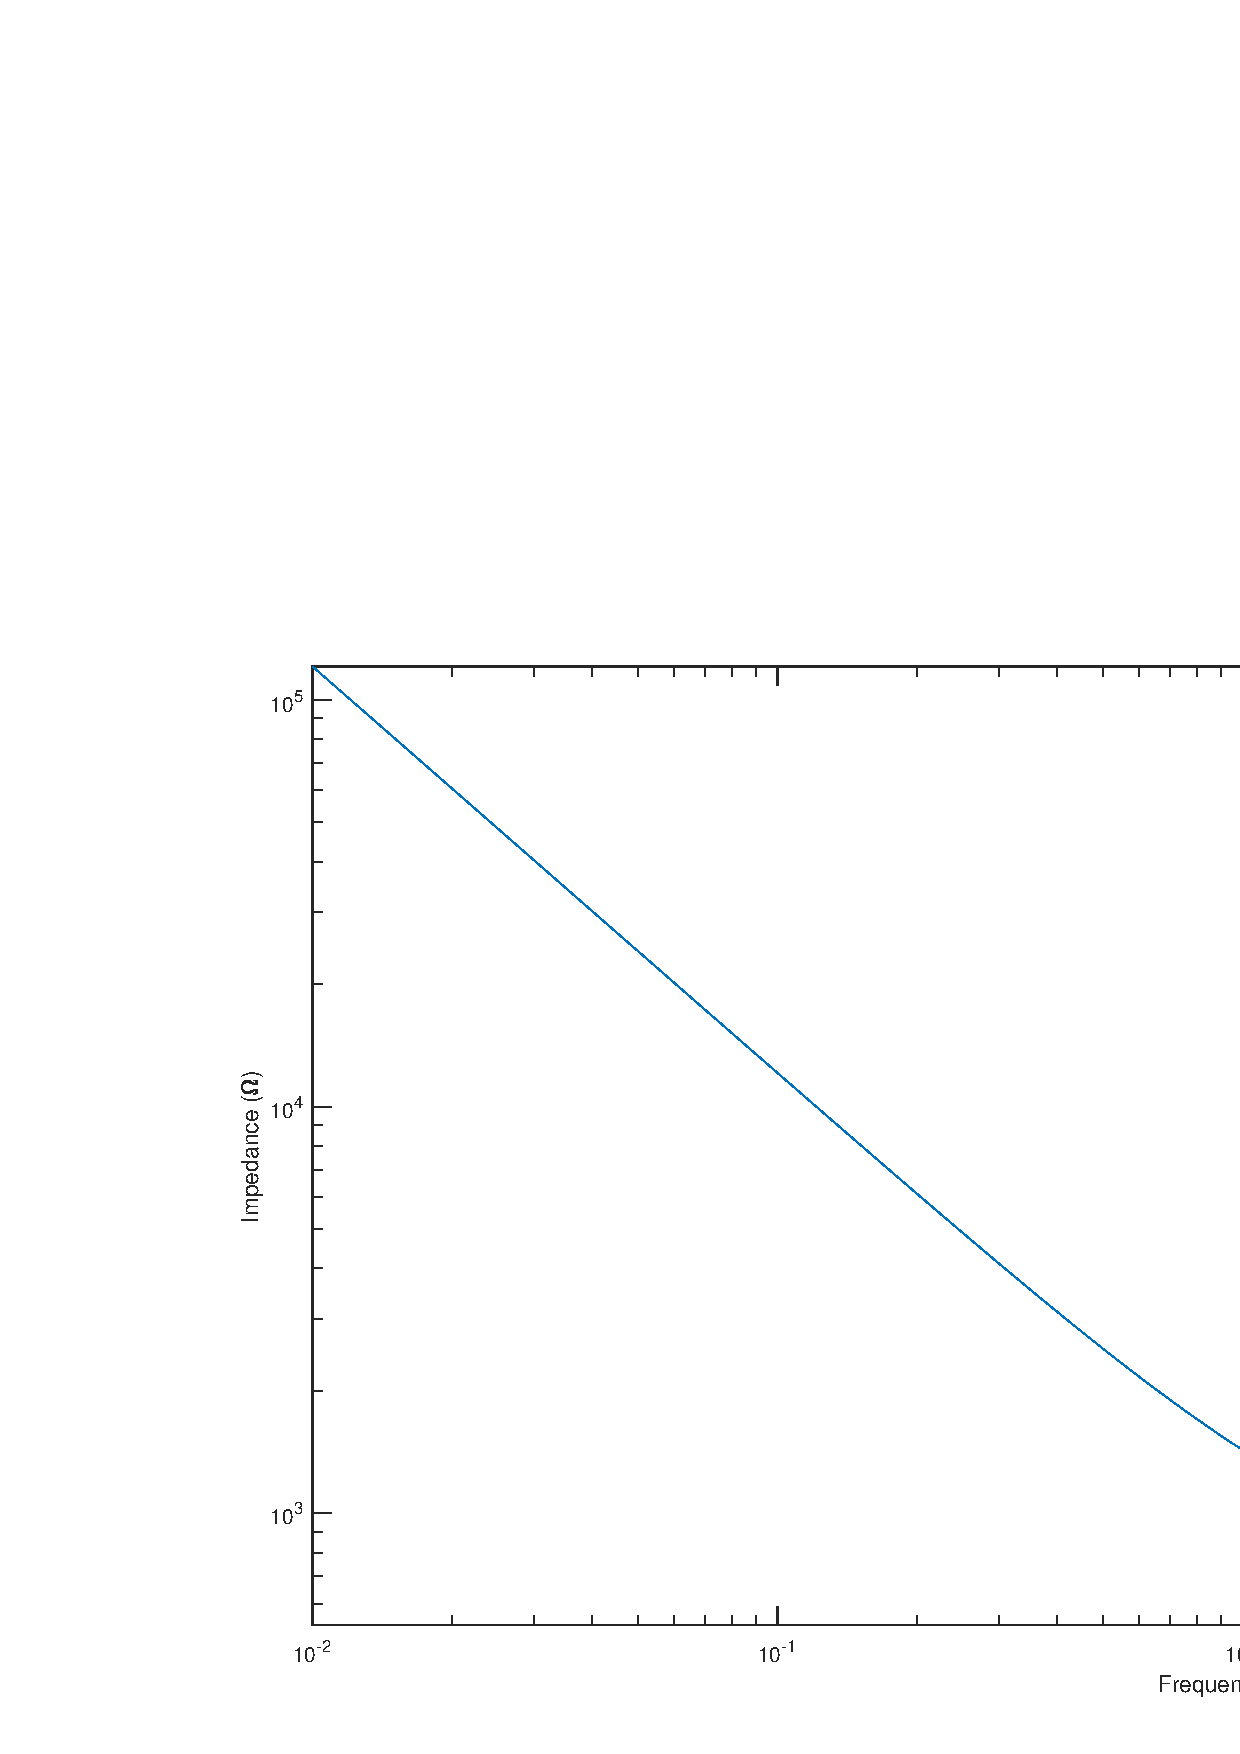
\includegraphics[width=\columnwidth]{3.png}
        \end{column}
        \begin{column}{0.4\textwidth}
            Inspired by the method we calculate the average power $P=UI*$, we can take the time average of the velocity by\\
            \[<v_{DL}>=\frac{1}{2}\mathrm{Re}\{\frac{\lambda_D\rho_{DL}E_{HL}^*}{\eta}\}\]
        \end{column}
    \end{columns}
\end{frame}
\begin{frame}{Velocity}
    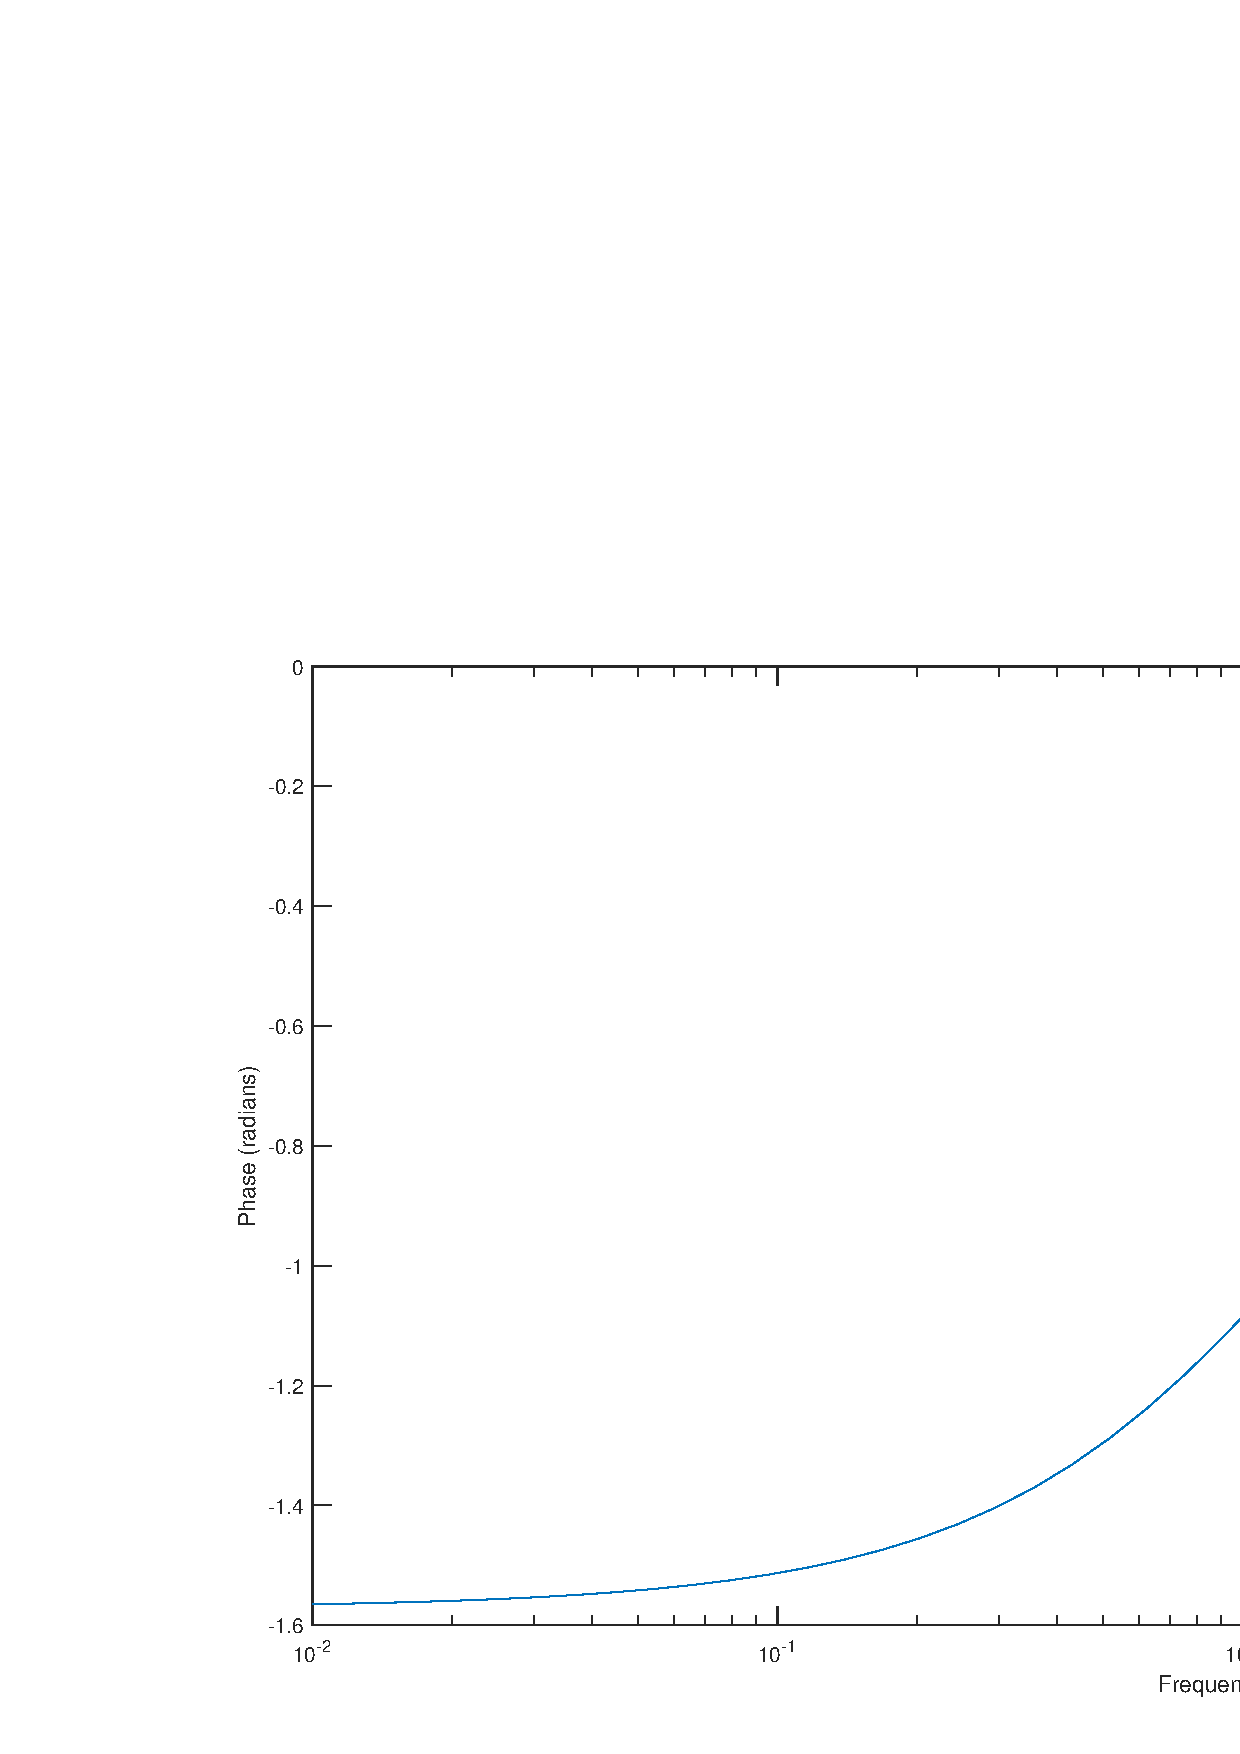
\includegraphics[width=0.6\linewidth]{4.png}
\end{frame}
\section{Unresolved Problem}
\begin{frame}{Unresolved Problem}
    According to previous calculation of total impedance,\\
    \[Z=\frac{\pi\left(\sqrt{k}+\frac{1}{\sqrt{k}}\right)}{2\sigma\ln{\frac{x_{max}}{x_{min}}}}+\frac{\varepsilon\left(x_{max}-x_{min}\right)}{\lambda_D\left(\sqrt{k}+\frac{1}{\sqrt{k}}\right)}\]
    However, the article gives a different result that\\
    \[Z=\frac{\pi\left(\sqrt{k}+\frac{1}{\sqrt{k}}\right)}{2l\sigma}\frac{\ln{A}-i\theta}{(\ln{A})^2+\theta^2}\]
    where
    \[A=\frac{\sqrt{\left[\left(2\lambda_D\sigma\right)^2+(\omega\varepsilon\pi)^2+x_{min}x_{max}\right]^2+\left[2\lambda_D\sigma\omega\varepsilon\pi\left(x_{max}-x_{min}\right)\right]^2}}{\left(2\lambda_D\sigma\right)^2+(\omega\varepsilon\pi x_{min})^2}\]
\end{frame}
\section{Velocity}
\begin{frame}{Velocity}
    \includegraphics[width=0.8\linewidth]{9.png}
\end{frame}
\section{Velocity}
\begin{frame}{Velocity}
    \begin{columns}[onlytextwidth]
        \begin{column}{0.45\textwidth}
            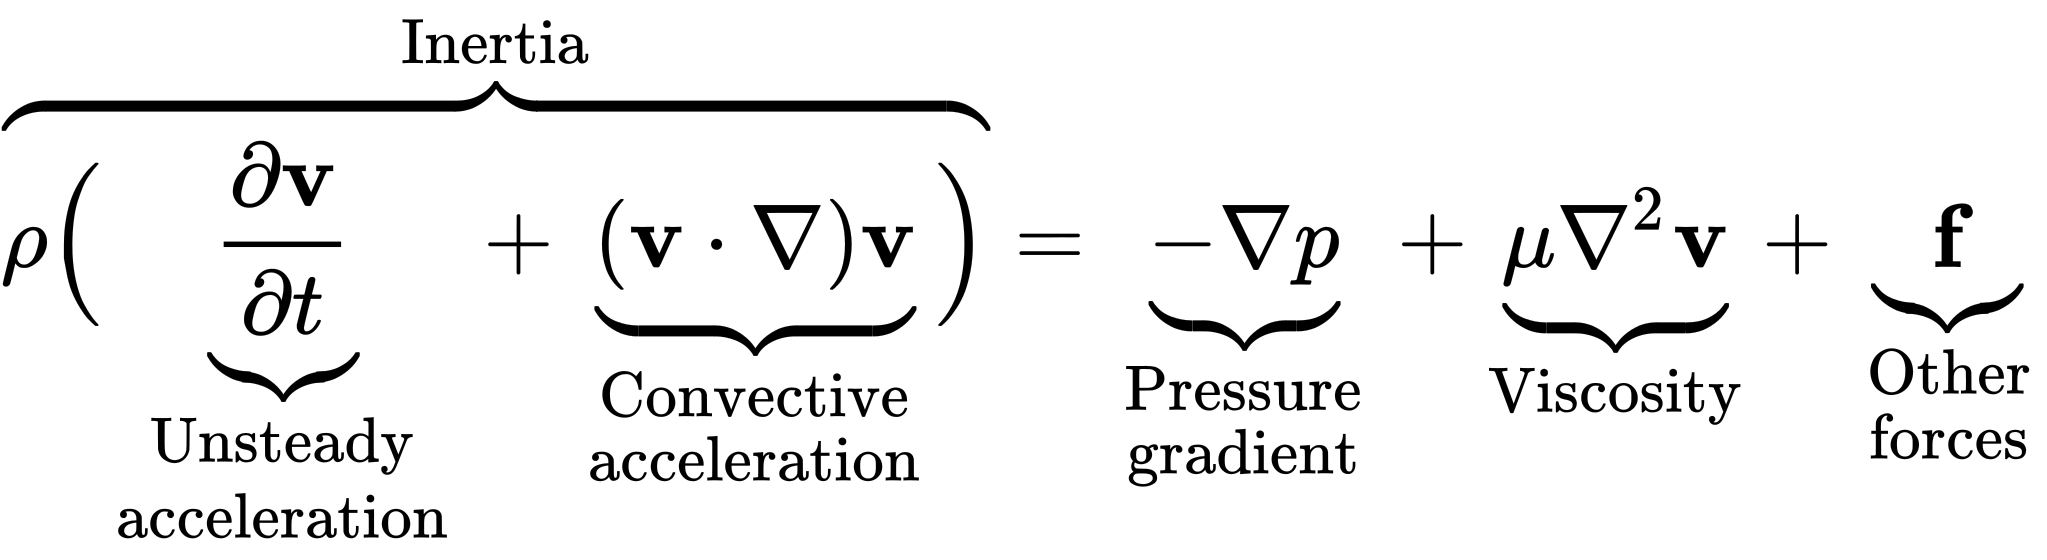
\includegraphics[width=\columnwidth]{7.png}
        \end{column}
        \begin{column}{0.45\textwidth}
            \includegraphics[width=\columnwidth]{8.jpg}
        \end{column}
    \end{columns}
\end{frame}
\begin{frame}{Unresolved Problem}
    and\\
    \[\theta=\arctan{\frac{2\lambda_D\sigma\omega\varepsilon\pi\left(x_{max}-x_{min}\right)}{\left(2\lambda_D\sigma\right)^2+(\omega\varepsilon\pi)^2x_{min}x_{max}}}\]
\end{frame}
\begin{frame}{Unresolved Problem}
    \begin{columns}[onlytextwidth]
        \begin{column}{0.35\textwidth}
            \includegraphics[width=\columnwidth]{5.png}
        \end{column}
        \begin{column}{0.55\textwidth}
            However, this does not match its figures.
            \includegraphics[width=\columnwidth]{6.jpg}
        \end{column}
    \end{columns}
\end{frame}
\end{document}